\documentclass{article}

% Language setting
% Replace `english' with e.g. `spanish' to change the document language
\usepackage[english]{babel}
\usepackage{hyperref}

% Set page size and margins
% Replace `letterpaper' with `a4paper' for UK/EU standard size
\usepackage[letterpaper,top=2cm,bottom=2cm,left=3cm,right=3cm,marginparwidth=1.75cm]{geometry}

% Useful packages
\usepackage{amsmath}
\usepackage{graphicx}
\usepackage[colorlinks=true, allcolors=blue]{hyperref}

\title{Verification of ACAS Xu using Alpha-Beta-Crown and Nnenum }
\author{Văduva Vlad-Andrei, Granu Dragoș Vlad, Iordache Constantin, Hrițu Toma\\[1cm]{\small Coordinator: Conf. dr. Erașcu Mădălina}}


\begin{document}
\maketitle
\newpage
\tableofcontents
\clearpage
\section{Abstract}
The purpose of verifying the ACAS Xu benchmark is to assure the correctness of the results output by the benchmark. Such results can have real life consequences. Therefore, it is important 
\section{Introduction}
ACAS Xu is an air-to-air collision avoidance system designed for unmanned aircraft that issues horizontal turn advisories to avoid an intruder aircraft. Due the use of a large lookup table in the design, a neural network compression of the policy was proposed. The purpose of this paper is to document the process of verifying the ACAS Xu benchmark using two VNN tools, alpha-beta crown and nnenum.
\section{ACAS Xu }
ACAS XU refers to the Automatic Collision Avoidance System - Experimental Upgrade. ACAS XU is a set of experimental enhancements to the existing ACAS II (Traffic Alert and Collision Avoidance System II) used in aviation. ACAS is a safety system designed to reduce the risk of mid-air collisions between aircraft.

ACAS II is based on the Traffic Advisory (TA) and Resolution Advisory (RA) concepts. When ACAS II detects a potential collision threat, it provides pilots with advisories to take evasive action, such as a vertical resolution advisory to climb or descend.

ACAS XU represents advancements and upgrades to the existing system, incorporating improved algorithms and technologies to enhance collision avoidance capabilities. It's important to note that developments in aviation technologies may have occurred since my last update, so you may want to check for the latest information to ensure accuracy.

\subsection{Architecture Elements}
ACAS Xu uses FC and Relu for its architecture.\newline
FC is a Fully Connected layer inside the neural network. This is one one the layer types that is used as a basis in almost all neural networks. In an FC layer, all the neurons of the input are connected to every neuron of the output layer. In an FC layer, a weighted linear transformation is applied to the input neurons and then pass the output through a non-linear activation function.
\newline
ReLU (Rectified Linear Unit) is an activation function that introduces the property of non-linearity to a deep learning model and solves the vanishing gradients issue.
\newpage
\section{Tools}
\subsection{Alpha-Beta-Crown}
Alpha-Beta-CROWN is a neural network verification tool based on an efficient linear bound propagation framework and branch and bound. It can be accelerated efficiently on GPUs and scales well for big convolutional neural networks.\newline
Supported neural network architectures:
\begin{itemize}
\item Layers: fully connected, convolutional, pooling, transposed convolution
\item Activation functions: ReLU, sigmoid, tanh, arctan, sin, cos, tan
\item Residual connections and other irregular graphs
\end{itemize}

Prerequisites: Conda, miniconda works as well
Miniconda Installation:
We create a folder named miniconda3:

\begin{verbatim}mkdir -p ~/miniconda3\end{verbatim}
We must download miniconda from the main site:
\begin{verbatim}wget https://repo.anaconda.com/miniconda/Miniconda3-latest-Linux-x86_64.sh -O ~/miniconda3/miniconda.sh\end{verbatim}
We run the installtaion script:
\begin{verbatim}bash ~/miniconda3/miniconda.sh -b -u -p ~/miniconda3
\end{verbatim}

After we installed the prerequisites, we can proceed with alpha-beta-crown installation:
We clone the GitHub repository:
\begin{verbatim}git clone --recursive https://github.com/Verified-Intelligence/alpha-beta-CROWN.git\end{verbatim}
This way, we also clone auto-LiRPA sub-module, which will then be installed with the command \begin{verbatim} python setup.py install\end{verbatim}
Remove the old environment, if necessary:
\begin{verbatim}conda deactivate\end{verbatim}
\begin{verbatim}conda env remove --name alpha-beta-crown\end{verbatim}

Install all dependents into the alpha-beta-crown environment:
\begin{verbatim}conda env create -f complete_verifier/environment.yaml --name alpha-beta-crown\end{verbatim}

Activate the environment
\begin{verbatim}conda activate alpha-beta-crown\end{verbatim}
To run alpha-beta-CROWN, we need to run abcrown.py, located in the complete\textunderscore verifier folder:
\begin{verbatim}
    python abcrown.py --config exp_configs/vnncomp23/acasxu.yaml
\end{verbatim}
Alpha-beta-CROWN will begin to verify the benchmark and at the end it will output a summary as such:\newline
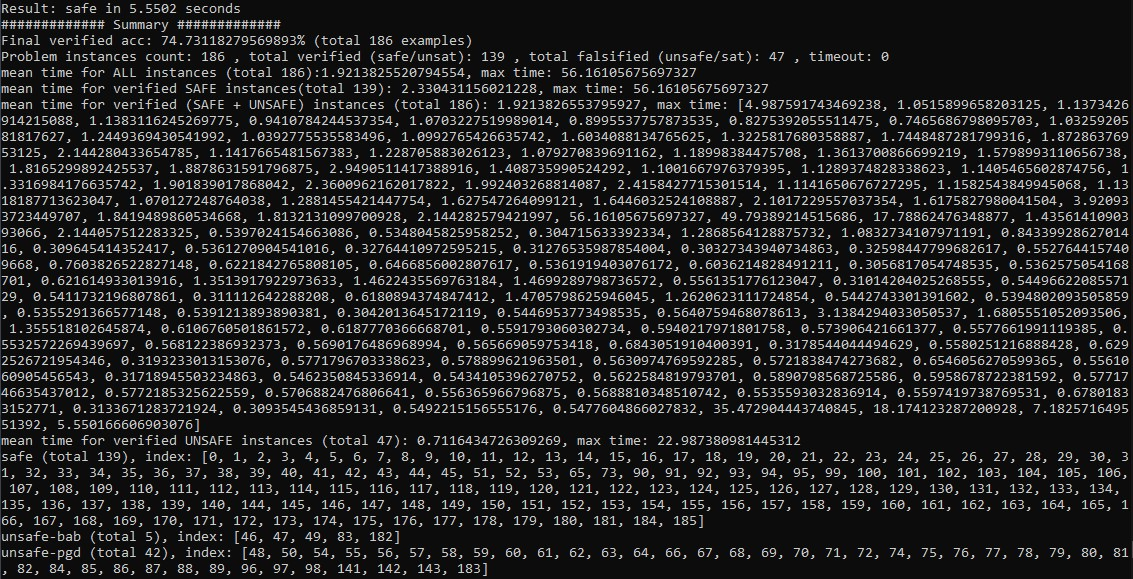
\includegraphics[scale=0.6]{alphabeta.jpg}

\subsection{Nnenum}
Prerequisites: 
\begin{itemize}
    \item Docker
    \item Python
\end{itemize}
To install nnenum, we first must clone the GitHub repository from the following address:  \url{https://github.com/stanleybak/nnenum}.
Next, we need to run the following command to build the tool using Docker:
\begin{verbatim}
    docker build . -t nnenum_image
\end{verbatim}
This will install all the prerequisites such as the required Python libraries.
\newline
Now that nnenum is installed, we can run it. First we need to run the following command:
\begin{verbatim}
    docker run -it nnenum_image bash
\end{verbatim}
This will start the shell in which nnenum is going to run.
\newline
In order to run onnx and vnnlib files one-by-one, we can use the follwing command from within this shell:
\begin{verbatim}
    python3 -m nnenum.nnenum examples/acasxu/data/ACASXU_run2a_3_3_batch_2000.onnx examples/acasxu/data/prop_9.vnnlib
\end{verbatim}
Alternatively, to run all the onnx and vnnlib files for ACAS Xu, we need to run the Python script located at examples/acasxu/acasxu\textunderscore all.py using the following command:
\begin{verbatim}
    python3 acasxu_all.py
\end{verbatim}
\clearpage

\section{Experimental Results}
\section{Conclusions}
\section{Bibliography}
\bibliography{sample}
\bibliographystyle{ieeetr}
\addcontentsline{toc}{chapter}{}


\end{document}